\chapter{Patient}
Ved implementering af en ny teknologi, herunder en Ultralyds Robotarm, kan det have en indvirkning på patienten. Derfor er det vigtig at belyse, hvilken effekt den nye teknologi har på patientgruppen. \\
I denne mini-MTV vil både gravide og sonografer blive placeret i rollen som patienter - gravide da de får foretaget en ultralydsscanning og sonografer da de er i risikogruppen for arbejdsskader. Begge grupper vil derfor blive belyst i dette afsnit.  \\ \newline
Dette afsnit vil delvist være baseret på interview og efterfølgende samtaler med sonografer på HEH og RMV. \textbf{Henvis via kilder istedet for} 
\newline
For at kunne udarbejde en fyldestgørende analyse af patientperspektivet er det nødvendigt at belyse flere forhold. Se figur \ref{patientMTV}, hvor de fem patientperspektiver er vist. 
\begin{figure}[h!]\centering
	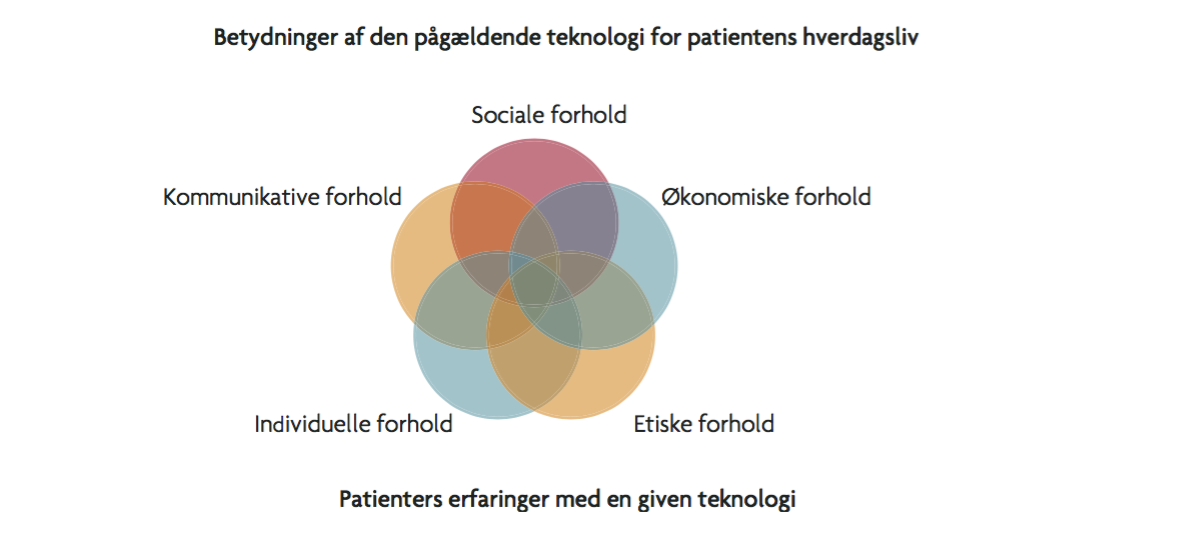
\includegraphics[width = 1.0\textwidth]{Figurer/PatientaspekterMTV}
	\caption{Udforskning af patientaspekter i MTV, som har betydning for patientens hverdagsliv. \cite{Leavitt}}
	\label{patientMTV}
\end{figure}

\textbf{Forklar hvor modellen giver mening}

\section{Sociale forhold}
På nuværende tidspunkt findes skepsis blandt sonografer i forhold til om de kan forsætte med at scanne indtil pensionsalderen. Der er lavet undersøgelser, som viser at 20 \% kommer på førtidspension grundet deres arbejde \cite{BeckyMorton2007}.  \\ 
For sonograferne vil eventuelle færre arbejdsskader betyde bedre fysiske funktioner i forhold til arbejde og fritid. Dette kan forlænge tiden på arbejdsmarkedet og forbedre personalemiljøet. \textbf{refrence til tidligere skrevet - noget med arbejdsglæde organisation}      

\section{Kommunikative forhold}
Produktet af scanningen, eksempelvis billeder og kønsbestemmelse, vil ikke blive påvirket af Ultralyds Robotarmen.
For sonograferne vil det kræve en anden introduktion, da de ikke længere vil have fysisk kontakt med den gravide, dog er de stadig placeret i samme rum.  \\
Sonograferne vil igennem bedre arbejdsstillinger potentielt opleve et andet overskud til arbejdssituationen og patientkontakten.  

\section{Individuelle forhold}
Enkelte gravide patienter kan opleve en utryghed ved at få en fremmed teknologi, robotarmen, fysisk tæt på sig. Dette kan forøge den utryghed, som den gravide i forvejen kan have i første trimester omkring sikkerheden af en ultralydsscanning \cite{Lea1985}. Der vil altid være en sonograf tilstede under en scanning, som skaber en menneskelig kontakt og en professionel tryghed.  \\
Sonografernes anciennitet vil være en stor tryghedsfaktor for patienten. Derved vil en eventuel utryghed fra den gravide patient blive mindsket når sonograferne udviser sikkerhed og åbenhed for teknologien. \textbf{hvad kender patienten til den enkeltes anciennitet}\\
For den gravide er det især vigtigt at knytte bånd med fosteret. Derved mener sonograferne på RMV, at så længe de gravide og deres pårørende kan følge med i scanningen på en skærm, vil den nye teknologi ikke have stor påvirkning på den gravide. \\  
Sonograferne er meget engagerede i deres arbejde, hvilket kan være en af grundene til, at de ikke indmelder skader. Dette er på trods af videnskabelige undersøgelser, som viser at mange sonografer døjer med smerter \cite{BeckyMorton2007}. 
Hvis akavede og fysisk udfordrende arbejdsstillinger for sonograferne undgås, kan det muligvis skabe en bedre opmærksomhed mod den gravide patient - eksempelvis overskud til forklaring af billeder og patientens velbefindende.  

\section{Etiske forhold}
\textbf{udtag aspekter som giver mest mening, Vigtig at udvælge til opgaven.}
Brugen af en Ultralyds Robotarm danner grundlag for en række etiske problemstillinger, som påvirker både gravide og sonografer. 
Problemstillingerne omhandler de professionsetiske principper \cite{Husted}: 
\textbf{tjek opstilling}
\begin{itemize}
	\item \textbf{Pligter}
	\begin{itemize}
		\item Undgå skade af brugeren:\\ 
		Ultralyds Robotarmen skal hverken være til skade for gravide eller sonograferne. 
	\end{itemize} 
	\item \textbf{Konsekvenser}
	\begin{itemize}
		\item Forebygge sygdom og sygelighed og fremme sundhed eller status quo: \\
		Hvis man ud fra et nytteetisk perspektiv, kan få flere gravide igennem en scanning på kortere tid og samtidig mindske antallet af arbejdsskader for sonografer, vil ressourcerne blive udnyttet bedst muligt, og derved komme flest mulige til gavn. Dette følger de socialetiske ideer i nytteetikken, som ud fra en overordnet forestilling ønsker at fremme nytte og retfærdighed for de mange.    
		\item Lindre lidelse, fremmedgørelse og ubehag:\\
		Ultralyds Robotarmen skal opfylde dette overfor både sonografer og patienten. Det kan tænkes, at patienten kan føle sig fremstillet som et objekt, fordi teknologien kommer tættere på patienten, mens sonograferne kommer længere væk. Dog er sonografen til stede i samme rum som patienten, derved er der stadig en form for menneskelig kontakt. Det kan tænkes at denne kontakt vil mindske risikoen for fremmedgørelse og ubehag for patienten.   
	\end{itemize}
	\item \textbf{Idealer}
	\begin{itemize}
		\item Handle med forståelse og empati:\\
		Ud fra patientens perspektiv kan det opfattes som en ændring af nærhed- og omsorgsrelationen mellem patienten og sonografen under en scanning med Ultralyds Robotarmen. 
		\item Handle med etisk ansvarlighed overfor sonografer:\\
		En af Ultralyds Robotarmens hovedfunktioner er at mindske antallet af sonografernes arbejdsskader. Derved skabes der en empati for sonografernes arbejdssituationen.\\
		Resultatet er at en mindskelse i antallet af arbejdsskader vil fremme personalesikkerhed og -trivsel.   		
	\end{itemize} 
\end{itemize} 

\section{Økonomiske forhold}
Ultralyds Robotarmen kommer ikke til at have økonomisk indvirkning for den gravide patient. Derimod ligger betalingen og andre tilkoblede ydelser ved den pågældende afdeling og dens ledelse. Dette uddybes i afsnittet Økonomi \ref{Okonomi}. \\
\textbf{økonomisk indvirkning på sonograferne}
Både på HEH og RMV ser sonograferne fordele ved Ultralyds Robotarmen, dog menes det, at økonomien og ledelsens beslutninger vil blive vægtet tungere end sonografernes argumenter.  
 
\section{Delkonklusion }
Set fra de patientmæssige forhold, vil indførslen af en Ultralyds Robotarm ikke have en stor indflydelse på de gravide. Den usikkerhed og eventuelle ubehag, der kan fremkomme, kan afhjælpes af sonografernes anciennitet (tilgang til opgaven). Så længe den gravide har mulighed for at danne et forhold til fosteret, burde de gravide ikke have et problem med det nye udstyr. 
Set fra sonografernes synsvinkel kan indførslen af Robotarmen forbedre deres arbejdsforhold. 